\documentclass[sigconf, natbib=false]{acmart}
\settopmatter{printacmref=false}
\renewcommand\footnotetextcopyrightpermission[1]{}
\acmConference[Software Engineering für AI-/ML-Systeme]{}{Juli 2026}{Rostock, Deutschland}
\usepackage{lipsum}
\usepackage[utf8]{inputenc}
\usepackage[T1]{fontenc}
\usepackage[ngerman]{babel}
\usepackage{graphicx}
\usepackage{subcaption}
\hypersetup{colorlinks, citecolor=BrickRed, filecolor=Black, linkcolor=Black, urlcolor=MidnightBlue}
\usepackage[normalem]{ulem}
\usepackage[backend=biber,bibencoding=utf8,urldateusetime=true,style=alphabetic,sorting=nyt,natbib=true]{biblatex}
\addbibresource{refs.bib}

\title{Report zur Präsentation -- Surprise Adequacy}

\author{Malte Grube}
\affiliation{
  \institution{Universität Rostock}
  \city{Rostock}
  \country{Deutschland}
}
\email{malte.grube@uni-rostock.de}

\begin{document}

\maketitle

\section{Sinn von Surprise Adequacy}
In der Softwareentwicklung ist es üblich, strukturierte Metriken wie Branch- oder Statement-Coverage zu verwenden, um die Qualität von Testfällen zu bewerten. In neuronalen Netzen (NNs) gibt es jedoch keine solchen Kontrollflussstrukturen. Somit sind diese Metriken nicht direkt anwendbar \cite{sa_2}.

Als frühere Metrik zählt die Neuron Coverage (NC) \cite{neuron_coverage}. Sie erfasst die Anzahl an Neuronen eines NN, die für die Testdaten einen bestimmten Schwellenwert überschreiten. Diese Metrik ist jedoch nicht fein genug, da die kontinuierlichen Aktivierungen von Neuronen hierbei nicht berücksichtigt werden \cite{sa_1,sa_2}.

Surprise Adequacy (SA) \cite{sa_1,sa_2} misst stattdessen, wie ''überraschend'' eine neue Eingabe für ein neuronales Netzwerk im Vergleich zu den \textit{Trainingsdaten} ist. Dabei werden Activation Traces (ATs) für eine Schicht des Netzwerks betrachtet, für jedes einzelne Input-Bild. Dieser Trace ist ein Vektor, der die Aktivierungen der Neuronen für den Input darstellt. Die Autoren \cite{sa_1,sa_2} empfehlen zudem, dass ein gutes Test-Set neben trainings-ähnlichen Daten auch stark abweichende oder gar adversariale Daten (e.g.\,manipulierte Bilder via FGSM) enthalten sollte. Mittels SA wurde schließlich geprüft, wie vielfältig eine Test-Suite ist, um die Abdeckung des möglichen Input-Spektrums zu ermitteln.

\section{Funktionsweise von SA}
SA wird für jeden einzelnen Test-Input basierend auf dem individuellen AT berechnet. Die Berechnung erfolgt der Einfachheit halber für eine ausgewählte Schicht, da die Aktivierungen einer Schicht einen Vektor bilden, der als AT bezeichnet wird.

Bezüglich SA gibt es verschiedene Varianten, welche sich in der Berechnung unterscheiden. Im ersten Paper von \cite{sa_1} werden Likelihood-based Surprise Adequacy (LSA) und Distance-based Surprise Adequacy (DSA) vorgestellt. Im zweiten Paper \cite{sa_2} wird zusätzlich die Mahalanobis Distance-based Surprise Adequacy (MDSA) vorgestellt, welche deutlich effizienter zu berechnen ist. 

\subsection{LSA}

LSA basiert auf der klassenweisen Schätzung der Wahrscheinlichkeitsdichte von ATs mittels Kernel Density Estimation (KDE). Die Dichte wird initial für die ATs der Trainingsdaten geschätzt. Für einen neuen Test-Input wird der AT extrahiert und in der Dichtefunktion ausgewertet. Folglich wird die Überraschung basierend auf der Dichte berechnet: $$LSA(x)=-\log(\hat{f}(x)).$$ Das bedeutet, je unwahrscheinlicher der Test-AT laut den Trainingsdaten ist (je kleiner die Dichte), desto größer ist das Ergebnis des negativen Logarithmus. Somit sind diese Inputs überraschender, da sie ein ungewöhnliches Aktivierungsmuster aufweisen, welches bei Trainingsdaten selten oder gar nicht vorgekommen ist \cite{sa_2}.

\subsection{DSA}

Um für DSA die klassenspezifische Überraschung des Test-Inputs zu berechnen, werden zwei Werte benötigt: Zuerst wird für das gegebene Testbild die euklidische Distanz im AT-Raum zum nächsten Trainings-AT ($\text{dist}_a$) der gleichen Klasse berechnet. Dann wird die Distanz vom selben Trainings-AT zum nächsten Trainings-AT einer fremden Klasse ($\text{dist}_b$) berechnet. DSA ist folglich das Verhältnis dieser beiden Distanzen: $$DSA(x)=\frac{\text{dist}_a}{\text{dist}_b}.$$ Je nachdem, wie nah der Test-AT an der Entscheidungsgrenze liegt, desto höher ist grundlegend die DSA \cite{sa_2}.

\subsection{MDSA}

Zur Berechnung von MDSA wird einmalig der Mittelwertsvektor $\mu$ und die Kovarianzmatrix $C$ aller Trainings-ATs berechnet. Für einen neuen Test-AT werden diese Elemente genutzt, um die Mahalanobis-Distanz zu berechnen: $$MDSA(x)=\sqrt{(x-\mu)^T C(x-\mu)}.$$ Liegt der Test-AT nah am Zentrum (Mittelwert) der Trainingsdaten, ist die MDSA niedrig, was als bekanntes Muster interpretiert wird. Liegt der Test-AT weit entfernt, ist die MDSA hoch, was auf ein unbekanntes oder manipuliertes Muster hindeutet. 

MDSA wurde als neue Metrik nach LSA und DSA vorgestellt, und ist deutlich schneller als die beiden Metriken, weil die ständigen Vergleiche zwischen neuem Input und den Trainingsdaten entfallen. Dadurch können industrielle Datensätze wie ImageNet sowie große Modelle mittels SA bewertet werden. Bereits das Sampling von 10\% der Trainingsdaten reicht bei ImageNet aus, um korrekte Rankings der Test-Inputs zu erhalten, was mit dem größten Speed-Up für MDSA von >9.0 einhergeht \cite{sa_2}.

\subsection{Surprise Coverage}

Im Gegensatz zu NC -- Zählung der Neuronen über den Schwellenwert für Test-Inputs -- bewertet die Surprise Coverage (SC) die Diversität einer gesamten Test-Suite unter Nutzung der SA-Werte. Nach der Berechnung der SA-Werte aller Test-Inputs wird der kontinuierliche Wertebereich in $n$ Buckets bis zu einer Obergrenze $U$ unterteilt. Somit wird der Wertebereich auf $(0,U]$ beschränkt. 

Die SC wird wie folgt ermittelt: Es wird gezählt, in wie viele dieser Buckets mindestens ein Test-Input der Suite fällt, basierend auf dem SA-Wert der Inputs. Anschließend wird diese Anzahl durch die Gesamtzahl der Buckets geteilt, wodurch ein Wert zwischen 0 und 100\% herauskommt. Ein hoher SC-Wert bedeutet, dass die Test-Suite eine hohe Diversität aufweist, aufgrund der hohen Anzahl an Buckets, die durch die Test-Inputs abgedeckt werden.

\section{Hands-on-Beispiel -- DSA mit MNIST} \label{sec:hands_on}
In der Präsentation wurde ein zweidimensionales Hands-on-Beispiel für DSA vorgestellt. Angenommen, es wurden klassenweise für eine bestimmte Modell-Schicht alle ATs für die Trainingsdaten berechnet. Ziel ist es, mit den ATs folglich die DSA-Werte für (1) ein Testbild und für (2) ein FGSM-Bild der Ziffer ''5'' zu berechnen. Nah zu diesen beiden Bildern liegen die ATs (3) einer ''5'' und (4) einer ''6'' aus den Trainingsdaten. Deren ATs werden berechnet und mit den Trainings-ATs verglichen, um die DSA-Werte zu ermitteln. Die Beispielvektoren sind wie folgt gegeben:
\begin{enumerate}
    \item Der Test-AT für ''5'': $(3,2)$
    \item Der FGSM-AT für ''5'': $(10,8)$
    \item Nächster Trainings-AT für ''5'': $(2,2)$
    \item Nächster Trainings-AT für fremde Klasse ''6'': $(6,2)$
\end{enumerate}
Mit diesen ATs können die DSA-Werte für beide Eingabe-Bilder mittels Euklidischer Distanz berechnet werden. Zuerst wird die Distanz vom neuen Test-AT der Zielklasse ''5'' zum nächsten Trainings-AT dieser Zielklasse berechnet ($\text{dist}_a$). Dann wird die Distanz vom selben Trainings-AT der Zielklasse zum nächsten Trainings-AT der fremden Klasse ''6'' berechnet ($\text{dist}_b$). DSA ergibt sich aus dem Verhältnis dieser beiden Distanzen:
\begin{align*}
\text{Testbild:} \quad \text{dist}_a &= \sqrt{(3-2)^2+(2-2)^2} = \textbf{1} \\
\text{dist}_b &= \sqrt{(6-2)^2+(2-2)^2} = \textbf{4} \quad \uuline{DSA = \frac{1}{4} = 0.25} \\
\text{FGSM-Bild:} \quad \text{dist}_a &= \sqrt{(10-2)^2+(8-2)^2} = \textbf{10} \\
\text{dist}_b &= \sqrt{(6-2)^2+(2-2)^2} = \textbf{4} \quad \uuline{DSA = \frac{10}{4} = 2.5}
\end{align*}
Das Testbild hat durch die Nähe zum Trainings-AT der Klasse ''5'' eine niedrige DSA von 0.25. Der AT ist somit ähnlich zu denen der Trainingsdaten, was eine geringe Überraschung folgert. Das FGSM-Bild hingegen hat eine 10-Mal so hohe DSA von 2.5, da es weiter von den Trainings-ATs der Zielklasse ''5'' entfernt ist, und näher an den ATs der fremden Klasse ''6'' liegt. Der AT des FGSM-Bildes ist somit weniger gewöhnlich im Vergleich zu den Trainingsdaten.

\begin{figure}[!ht]
    \centering
    \setlength{\belowcaptionskip}{-2em}
    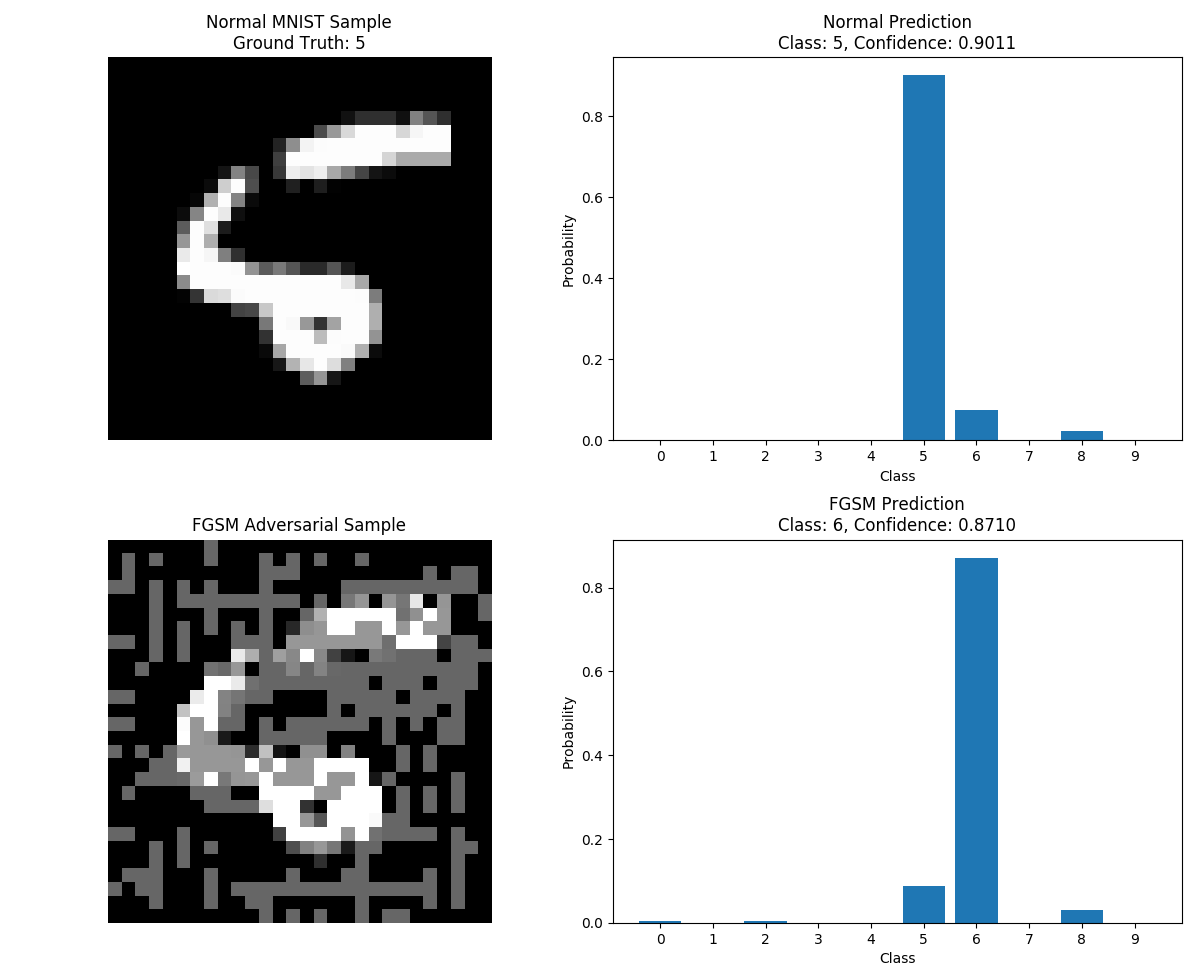
\includegraphics[width=.925\linewidth]{img/prediction_5.png}
    \caption{Vorhersage einer ''5''. Das Test-Bild wurde mit hoher Wahrscheinlichkeit korrekt klassifiziert, während das FGSM-Bild stattdessen als ''6'' klassifiziert wurde.}
    \label{fig:comparison}
\end{figure}

Dies kann zu Fehlklassifikationen führen, da ungewöhnliche ATs für FGSM-basierte Bilder vorliegen. Als Beispiel dient Abbildung \ref{fig:comparison}. 

\section{Repository-Beispiel -- LSA mit MNIST}
Die offizielle Implementierung von SA\footnote{\url{www.github.com/coinse/sadl}, letzter Zugriff 04/05/2026} bietet die Möglichkeit, beispielsweise LSA auf dem MNIST-Datensatz anzuwenden. Das Repository bietet unter anderem eine Trainings-Pipeline für ein einfaches Convolutional Neural Network (CNN) sowie die Berechnung von LSA für Test- oder FGSM-Bilder. Es wurde für den Report mit Python 3.5.10, pip 9.0.1 und \textit{Linux 6.19.11-arch1-1} getestet.

Bereits 3 Epochen (statt 50 wie im Repository) an Training mit dem gegebenen 5-Schichten-CNN haben für MNIST ausgereicht, eine Validation Accuracy von 98.78\% zu erreichen. Danach wurden die ATs für Trainings-, Test- und FGSM-Bilder berechnet, um anschließend die LSA-Werte für Test- und FGSM-Bilder -- hinsichtlich des Training-Sets -- zu ermitteln. Die Geschwindigkeit der LSA-Berechnung wurde verbessert, indem im Code durch die Autoren irrelevante Neuronen, basierend auf einem Schwellenwert \cite{sa_1}, herausgefiltert wurden. Im zweiten Paper \cite{sa_2} wird empfohlen, dies auch auf DSA und MDSA anzuwenden, auch wenn es nicht zwingend erforderlich ist.

Ein Vergleich der LSA-Werte für Test- und FGSM-Bilder zeigt, dass die FGSM-Bilder klassenweise oftmals breiter und nach rechts verschoben verteilt sind, was eine Tendenz zu höheren LSA-Werten aufweist (siehe Abbildung \ref{fig:lsa_classes}). Der Mean für Test beträgt -52.31, während FGSM einen Mean von 5.53 aufweist. In Abbildung \ref{fig:lsa_comparison} wirken die akkumulierten Ergebnisse für LSA nicht bahnbrechend, zumal ausschließlich LSA getestet wurde. DSA oder gar MDSA wurden hingegen nicht getestet, da in diesem Repository LSA mit MNIST als primäres Beispiel schnell anwendbar ist.

Hinsichtlich der SC weist die Vermischung beider Datensätze einen höheren Wert auf. Die Test-Suite zeigt lokale 27.7\% SC, während die Kombination aus Test- und FGSM-Bildern 31.7\% SC aufweist. In \cite{sa_2} wurde die SC für LSA durch weitere Adversarial-Datensätze auf bis zu 71\% erhöht, was die Diversität der Test-Suite deutlich steigert. Aufgrund der 3 Epochen an Training fallen die SC-Werte von den Ergebnissen etwas geringer als in \cite{sa_1} aus. Mehr Informationen zum Repository gibt es im Anhang \ref{sec:code}.

\section{Schlusswort}
Die Ergebnisse zu SA verdeutlichen, dass eine systematische Auswahl an Bildern über das LSA-Spektrum hinweg (von ähnlich zu Trainingsdaten bis hin zu stark abweichend) sinnvoll sein kann, um das Modell mittels Retraining zu verbessern \cite{sa_1}. Das Nachfolgepaper \cite{sa_2} zeigt jedoch, dass der Retraining-Effekt in den umfassenderen Experimenten zu SA nicht allzu stark ist. SA reicht allein nicht aus, um ein gutes Retraining zu gewährleisten.

Es wird dennoch eine ausreichend schnelle Pipeline geboten, um beispielsweise LSA auf gängigen Datensätzen wie MNIST anzuwenden. Zuvor haben die Autoren das MNIST-Testset mit FGSM manipuliert, und dieses zur Verfügung gestellt, siehe Abbildung \ref{fig:comparison}.

Grundlegend kann SA ''überraschende'' Inputs erkennen, jedoch nicht erklären, warum ein Modell die Entscheidung für jene Inputs trifft, im Vergleich zu Explainable AI (XAI) Methoden. 

\pagebreak
\appendix
\setcounter{figure}{0}
\renewcommand{\thefigure}{\thesection.\arabic{figure}}

\section{LSA Histogramme}

Die folgenden LSA-Histogramme wurden zur besseren visuellen Differenzierung im positiven Bereich bis $x \leq 200$ dargestellt.

\begin{figure}[h]
    \centering
    \begin{subfigure}[b]{0.48\linewidth}
        \centering
        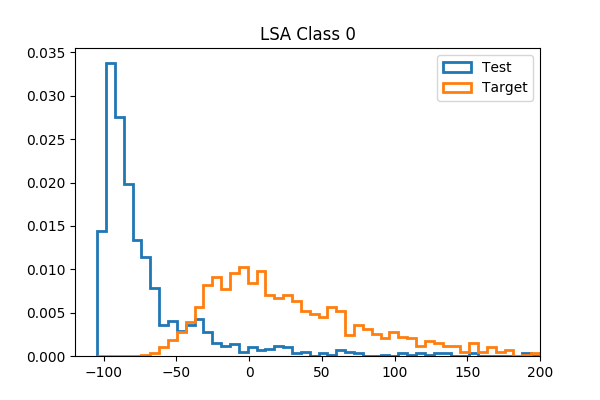
\includegraphics[width=\linewidth]{img/lsa_class_0.png}
        \caption{Klasse 0}
    \end{subfigure}\hfill
    \begin{subfigure}[b]{0.48\linewidth}
        \centering
        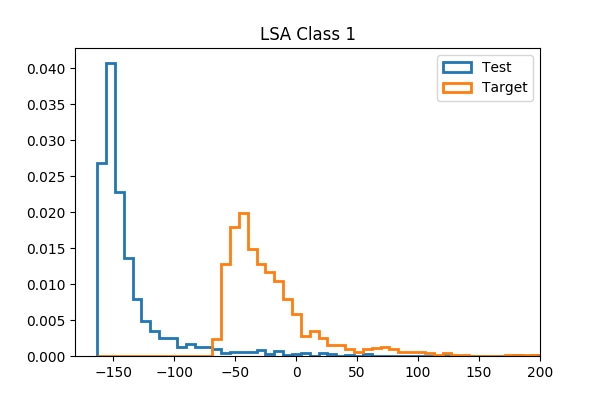
\includegraphics[width=\linewidth]{img/lsa_class_1.png}
        \caption{Klasse 1}
    \end{subfigure}
    
    \vspace{0.3cm}
    
    \begin{subfigure}[b]{0.48\linewidth}
        \centering
        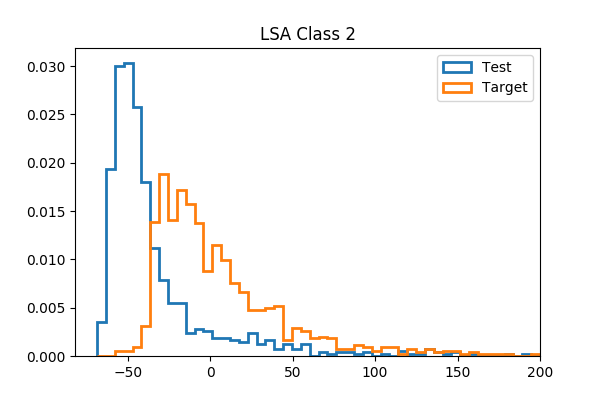
\includegraphics[width=\linewidth]{img/lsa_class_2.png}
        \caption{Klasse 2}
    \end{subfigure}\hfill
    \begin{subfigure}[b]{0.48\linewidth}
        \centering
        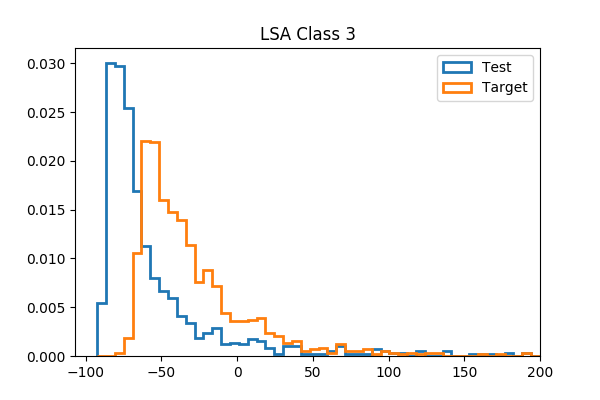
\includegraphics[width=\linewidth]{img/lsa_class_3.png}
        \caption{Klasse 3}
    \end{subfigure}

    \vspace{0.3cm}
    
    \begin{subfigure}[b]{0.48\linewidth}
        \centering
        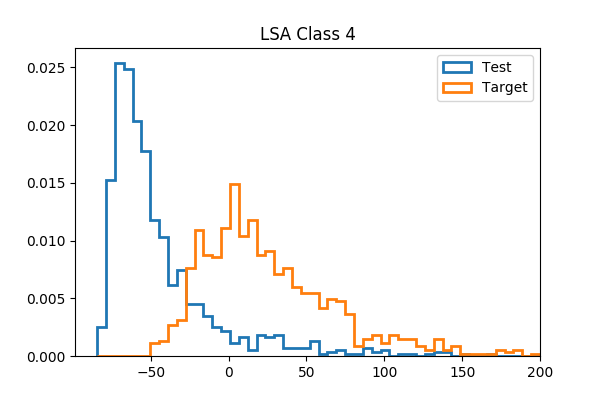
\includegraphics[width=\linewidth]{img/lsa_class_4.png}
        \caption{Klasse 4}
    \end{subfigure}\hfill
    \begin{subfigure}[b]{0.48\linewidth}
        \centering
        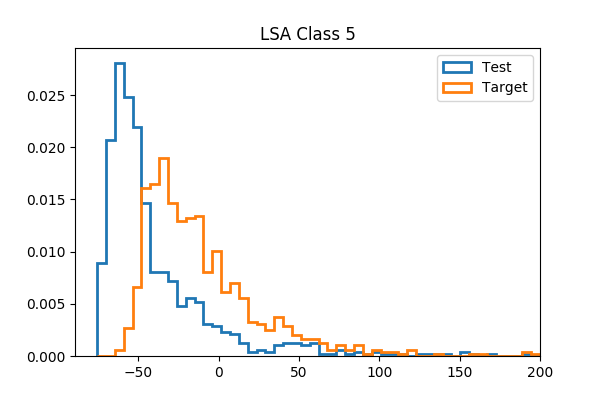
\includegraphics[width=\linewidth]{img/lsa_class_5.png}
        \caption{Klasse 5}
    \end{subfigure}

    \vspace{0.3cm}
    
    \begin{subfigure}[b]{0.48\linewidth}
        \centering
        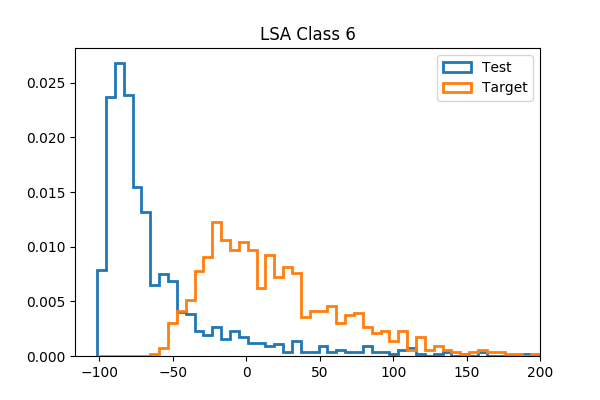
\includegraphics[width=\linewidth]{img/lsa_class_6.png}
        \caption{Klasse 6}
    \end{subfigure}\hfill
    \begin{subfigure}[b]{0.48\linewidth}
        \centering
        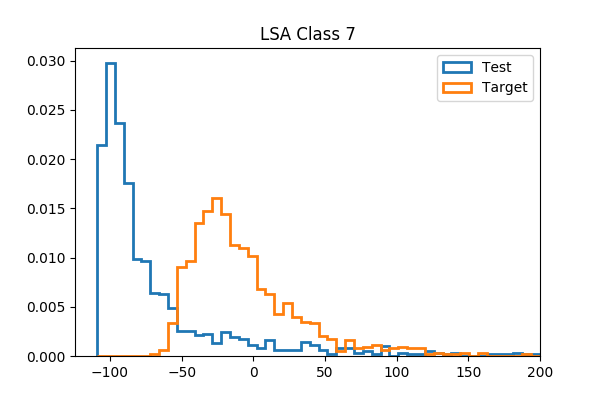
\includegraphics[width=\linewidth]{img/lsa_class_7.png}
        \caption{Klasse 7}
    \end{subfigure}

    \vspace{0.3cm}
    
    \begin{subfigure}[b]{0.48\linewidth}
        \centering
        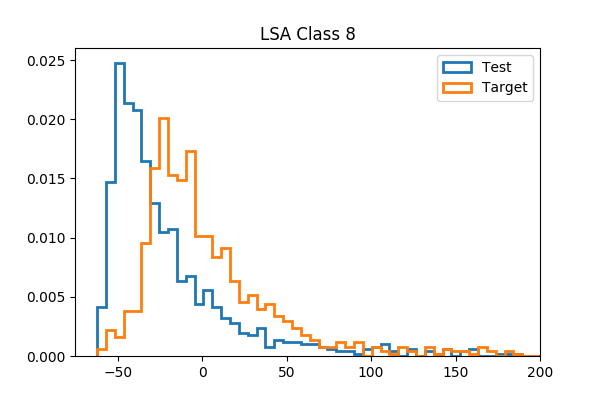
\includegraphics[width=\linewidth]{img/lsa_class_8.png}
        \caption{Klasse 8}
    \end{subfigure}\hfill
    \begin{subfigure}[b]{0.48\linewidth}
        \centering
        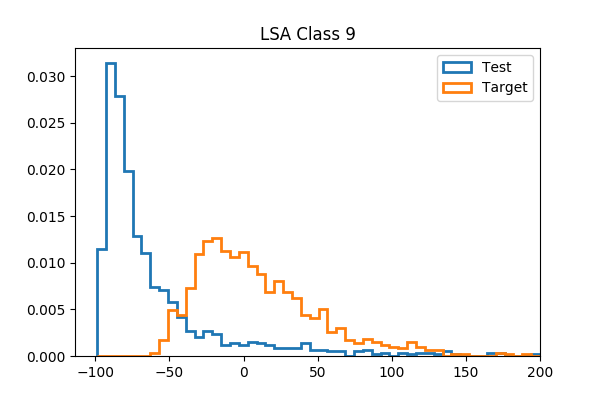
\includegraphics[width=\linewidth]{img/lsa_class_9.png}
        \caption{Klasse 9}
    \end{subfigure}
    
    \caption{Übersicht der LSA-Histogramme pro MNIST-Klasse (0-9) für das Testset. Die LSA-Verteilungen sind zum Vergleich pro Klasse sowohl für originale als auch FGSM-manipulierte Bilder dargestellt.}
    \label{fig:lsa_classes}
\end{figure}

\vfill\eject

\begin{figure}[h]
    \centering
    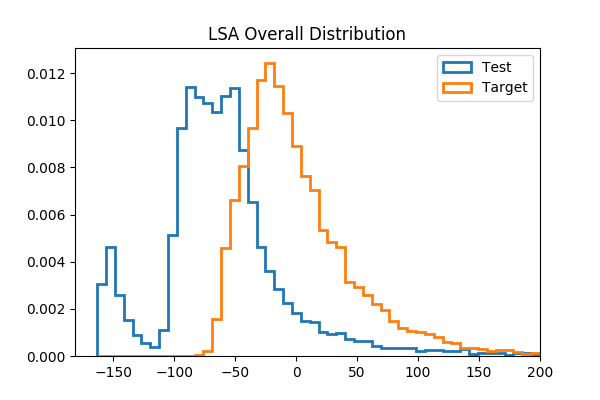
\includegraphics[width=0.65\linewidth]{img/lsa_overall.png}
    \caption{Akkumulierte LSA-Verteilungen für das MNIST-Testset zwischen Original- und FGSM-Bildern.\vspace{-1em}}
    \label{fig:lsa_comparison}
\end{figure}

\section{Zum Source Code} \label{sec:code}

Der Code zum Report befindet sich in einem GitHub-Fork\footnote{\url{https://github.com/mgrube753/sadl-se4ai}} zur offiziellen Implementierung. Es wurden Anpassungen vorgenommen, um beispielsweise das \textbf{fehlende} \texttt{Tensorboard}-Logging für das Training, für die LSA- und SC-Berechnungen zu ermöglichen, siehe Abbildungen \ref{fig:lsa_classes} und \ref{fig:lsa_comparison}. Zudem wurde ein Python-Modul (\texttt{show\_examples.py}) hinzugefügt, um die Vorhersage aus Abbildung \ref{fig:comparison} zu präsentieren. Änderungen zum Originalcode sind durch Beginn- und End-Kommentare markiert (sowie durch Git Diffs ersichtlich), vorwiegend in \texttt{run.py} zu finden.

Wie in \cite{sa_1,sa_2} angegeben, kann sich die SA-Berechnung auf anderen DL-Architekturen abweichend verhalten, wie im jeweiligen ''Threats to Validity'' Kapitel zu sehen. Daraus ergibt sich die Frage, wieso viele Aspekte nicht in der Implementierung berücksichtigt wurden, da diverse Paper-Details darin nicht abgedeckt wurden. Jegliches Seed-Management für eine \textit{geeignete Reproduzierbarkeit} der Ergebnisse ist zudem nicht implementiert worden, weshalb die Ergebnisse des Reports nicht mit den Ergebnissen im Paper übereinstimmen können. Dies gilt sowohl für das durchgeführte 3-Epochen-Training (ausreichende Validation Accuracy), als auch für ein womöglich verlangtes 50-Epochen-Training. Die Anzahl der Epochen wurde in den Papern nicht dargelegt, aber die standardmäßigen 50 Epochen sollten korrekt sein. Jegliche Ergebnisse können trotzdem anders ausfallen, da die Modellparameter entscheidend für die SA-Werte sind. Des Weiteren ist das Ermitteln von SC-Werten nur teilweise implementiert worden: entweder wird die Coverage für die gesamte Test-Suite oder für die gesamte FGSM-basierte Suite bestimmt. Keinerlei Kombination beider Suiten (wie in beiden Veröffentlichungen) ist möglich gewesen. Dies musste eigenständig hinzugefügt werden. Die Werte bezüglich des 3-Epochen-Trainings sind etwas geringer als in \cite{sa_1}, aber zeigen ähnliche Tendenzen.

Die Autoren haben zudem, im Gegensatz zum geringfügig abdeckenden Material, in ihren Papern weitere Adversarial-Datensätze (wie BIM, JSMA, ...) vorgestellt, um schrittweise die SC-Werte zu erhöhen. Dies geschah durch iteratives Hinzufügen von 1.000 manipulierten Bildern pro Adversarial-Datensatz (Test+FGSM $\to$ $\cdots$+BIM-A, etc.) \cite{sa_1}. Im Repository werden lediglich entweder alle 10.000 FGSM-Bilder oder Test-Bilder auf einmal betrachtet, ohne eine Vermischung beider Sets. Zusammenfassend, viele Paper-Details wurden nicht im Repository abgedeckt, und wurden teilweise eigenständig hinzugefügt, um ausreichend demonstrieren zu können.

\pagebreak

\printbibliography

\end{document}